\documentclass[twoside,leqno,twocolumn]{article}


\usepackage[charter]{mathdesign}
\usepackage{fullpage}
%\usepackage{amssymb}
\usepackage{amsmath}
\usepackage{verbatim}
\usepackage{ifthen}
\usepackage{url}
\usepackage{xspace}
% \usepackage[edges]{forest}
\usepackage{subcaption}
\usepackage{amsthm}
\usepackage{calrsfs}
\usepackage{hyperref}
\hypersetup{colorlinks=false,raiselinks=false,breaklinks=true}
\hypersetup{pdfborder={0 0 0}}
\hypersetup{bookmarksnumbered=true}
\usepackage{authblk}
\usepackage[show]{notes}


\title{CS-E4870 \\
        \large Research Project in Machine Learning and Data Science} 
\author{Ananth Mahadevan} 
\affil{Department of Computer Science, Aalto University\\
\href{mailto:ananth.mahadevan@aalto.fi}{ananth.mahadevan@aalto.fi}}


\date{}
\begin{document}
\maketitle

\begin{abstract}
    \label{sec:abstract}
    % Wikipedia is a well known online encyclopedia containing over 5 million pages of content. In contrast the number of active Wikipedia members who maintain all this information is relatively small. 
% For a Wikipedia member to rise to the level of an administrator, they or a nominator need to submit a request for Adminship (RfA). In this election any Wikipedia may cast a vote in support, opposition or neutral towards the candidate.
% This provides us with a very rich dataset on voting patterns withing Wikipedia members. The goal of this project is to collect data of such votes as well as data regarding individual Wikipedia member's contributions.
% This allows us to create and analyze networks of interactions among all Wikipedia users.
\begin{abstract}
    \label{sec:abstract}
\end{abstract}

\end{abstract}


% \begin{itemize}
%     \item how wikipedia is a large encyclopedia
%     \item maintained by a small group of Administrators
%     \item They undergo an election like process of RfAs
%     \item How this is an important online social election framework
%     \item How it has been studied in previous works 
%     \item What we aim to do by using a social network and theories of democracy
% \end{itemize}
\section{Introduction}
\label{sec:introduction}

Wikipedia is the largest online encyclopedia containing over 5 million pages of content. It is one the most popular websites on the Internet. Wikipedia has a diverse collection of articles from many different topics and is constantly being updated. Although Wikipedia started out as an open platform where anyone could create and articles, this lead to many factual errors and biased articles. Wikipedia started to incorporate elements hierarchy gradually over time. In the English version of Wikipedia all editors need to have a registered account and pages that are controversial and of a sensitive nature are protected by administrators.
\smallskip

Administrators are editors who are given access to tools such as blocking and unblocking other users, deleting and undeleting pages, protecting and renaming pages etc. Any user can \textbf{Request for Adminship}(RfA) in which the Wikipedia community participates. The RfA spans over seven days, during which any editor can comment and discuss the candidate. Editors scrutinize the candidate's contributions and credentials as well their conduct in the online discussion and overall experience. They can then state either their support or opposition to the candidate along with comments. At the end of seven days a Bureaucrat (an editor higher up in the hierarchy) decides on the consensus of the election and declare the outcome. Consensus is not a direct majority voting scheme and the final call rests with the Bureaucrat.
\smallskip

The RfA is a very intense and selective process, there are only 1400 total administrators of which only 500 are currently active\footnote{all data as of March 2020 for English version Wikipedia}. This is out of 38 million registered editors with only around 130 thousand are regular contributors. This small group of active administrators and editors are responsible for creating and maintaining all articles on Wikipedia.
\smallskip

Therefore the RfA process can give us valuable insight into the dynamics of social interactions and elections in an online platform. In this paper we will first discuss the existing work on studying the RfA elections and other such similar online processes. Next we provide an overview of the data collected and used from Wikipedia in this paper. We then present our main contribution, the use of a \textit{Viscous Democracy} to model the RfA election process. We discuss the results and possible extensions of this framework to other online elections systems.  


% For a Wikipedia member to rise to the level of an administrator, they or a nominator need to submit a request for Adminship (RfA). In this election any Wikipedia may cast a vote in support, opposition or neutral towards the candidate.
% This provides us with a very rich dataset on voting patterns withing Wikipedia members. The goal of this project is to collect data of such votes as well as data regarding individual Wikipedia member's contributions.
% This allows us to create and analyze networks of interactions among all Wikipedia users.



% \begin{itemize}
%     \item election prediction using candidate stats
%     \item election analysis using voter and candidate info
%     \item prediction using communication and how close 
%     \item Signed edge prediction and difficulties
% \end{itemize}
\section{Literature review}
\label{sec:literature-review}

The Wikipedia RfA process has been widely studied in various domains from many different perspectives such as those of the candidate, the voters, the community etc. In this section we discuss the existing work in this field.

Administrator is a highly coveted status on Wikipedia and there are many features than can be used to determine the worthiness of a candidate. Wikipedia themselves provide tools and guides\footnote{http://en.wikipedia.org/wiki/Wikipedia:GRFA} to help potential candidate assess their own electability. Wikipedia's \textit{admin score tool} as seen in Figure~\ref{fig:admin-score} uses features such as edit counts, pages created, age of account etc. Similarly, Burke et al. \cite{BurkeMoppingUp} utilized past RfAs to find features that correlate highly with success such as presence of edit summaries, politeness in user interactions and varied experience. Such tools and models are useful for finding potential nominees and understanding what the community values and respects. This however doesn't offer any insights into the dynamics that might play out in any particular election
\begin{figure}[h!]
    \centering
    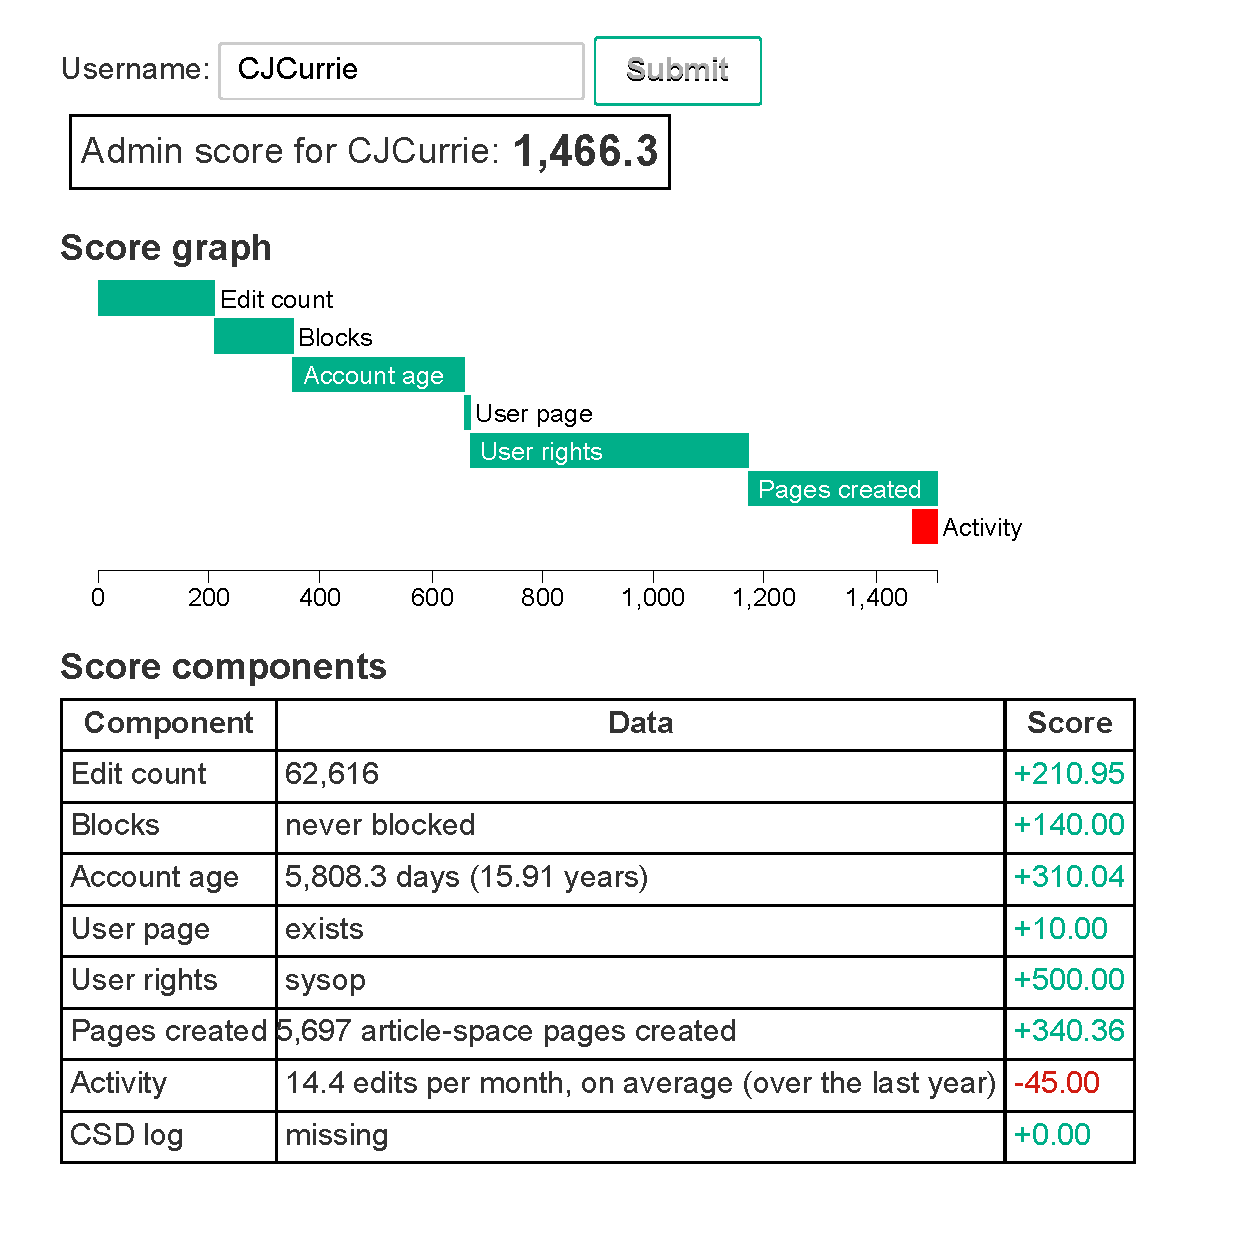
\includegraphics[width=\linewidth]{images/Asynchronous Admin Score.pdf}
    \caption{Admin score tool for user CJCurrie and it's breakdown}
    \label{fig:admin-score}
\end{figure}

Leskovec et al. provide a thorough analysis of the election from the perspective of the voter. They show that the voters make decisions based on \textit{relative assessment} of merit and degree of correspondence with the candidate. Elections do not follow a \textit{herd mentality} and standard information cascades. We see an interesting result that voters have diverse personal response functions as well as admin and non-admin patterns of voting differ. \cite{leskovec2010governance} We get a detailed picture of the temporal dynamics in a RfA.

As the votes in an RfA election can be positive or negative they can form a \textit{signed network} which has been studied and analyzed in great detail. We see that the Wikipedia RfA network has more compliance with status theory compared to balance theory in Leskovec et al. \cite{leskovecSigned}. When Leskovec et al. try and use these signed structural properties to predict edges in \cite{leskovecPredicting}, they see that the predictive accuracy is poor for Wikipedia RfA network compared to the other networks used. However as signed edge prediction methods are designed to work with any generic signed network, they tend to discard information that RfAs are elections and play out in a timely manner. Also predicting a single edge i.e a vote does not increase the accuracy in predicting the result of an election.   

The work of Desai et al. \cite{desai2014result} is related closely with the contributions presented in this paper. They use linear models for regression and classification to identify a core of \textit{influential voters} through feature selection. Using a set of 40 most influential voters they are able to predict the result of an election with a high accuracy. They also collect additional network features of the voters independent from the elections. Their results do not improve significantly in using the additional features in predicting election results. These results show that there are a group of influential voters that determine elections. This will be more evident when we analyze the dataset in coming sections.



\section{Dataset}
\label{sec:dataset}

We use two different types of data to help build the election model in this paper. The first would be information of the votes cast in a RfA and the eventual result of the RfA. This gives us the users interactions in an online election process where they have to judge their peers. The second, is information on the interactions of users in other non-elections settings. In Wikipedia discussions occur in \textit{Talk Pages}. Every type of Wikipedia page (articles, user pages, help pages etc.) has a \textit{Talk Page} where users can discuss the contents of that article or interact with the user or provide information to others. These are valuable data sources to gather more details on user activities.

In this section we will discuss the existing Wikipedia datasets from Stanford Network Analysis Project (SNAP) \cite{snapnets} that satisfy our requirements and their inherent limitations. Next we will illustrate the process by which we collected newer data from Wikipedia.


\subsection{Existing Datasets}
For the first type of data we require, there are two existing Wikipedia RfA datasets in SNAP namely \wikielect a
nd \wikirfa. They both contain attributes of each vote in a RfA such as the source, target, vote, result of RfA, timestamp. The \wikirfa is a more recent version of the \wikielect dataset. It has RfAs till May 2013 and also has the comment text of voters. There are 11,000 users and around 190 thousand votes in total. Both of these datasets have been used in many previous works mostly as signed networks. There are a few limitations of these datasets when we would like to analyse them as vote cast in an election. There is more than 5\% of \wikirfa votes that have no timestamp and almost 1\% of votes that have no source. As most RfAs have fewer than 300 votes this is an issue when considering the sequence of votes as well as who has cast a vote.

The interactions between users outside of RfA elections is useful to understand behaviour and perceptions of others. Wikipedia users can directly interact with another user by writing on their \textit{User Talk Page}. This can be a measure of how much correspondence exists between two users. We saw how this is a good indication of probability of supporting a candidate for an election \cite{leskovec2010governance}. The \textit{wiki-Talk} dataset on SNAP contains a directed network where an edge from node \textit{u} to \textit{v} signifies that \textit{u} has written in \textit{v}'s talk page. This dataset is a large network containing more than 2 million nodes and 5 million edges. The limitation of this network data is that nodes do not have user id mapping and also the edges are not weighted. Without a node to user id mapping the network cannot be used with the election data. Having weighted edges tells us how many times a user has interacted with someone else which is more informative. 
\smallskip

Due to the limitations of the existing datasets we set out to collect our own data to build our election model.

\subsection{RfA Data Collection}

We went through a 60GB XML dump of Wikipedia from Jan 2019 to extract the RfA data. We chose to scrape the data in a format similar to the SNAP \wikirfa dataset. The outline of the data extraction process is illustrated in Figure~\ref{fig:rfa-extraction}. In the first step we filter out all Wiki pages whose title doesn't contain the term \texttt{Requests for adminship}. This still leaves us with a lot of non-election Wiki pages, so we can further filter by checking for terms such as \texttt{Category:Unsuccessful requests} or \texttt{Category:Successful requests}.Now this reduces the space from over 5 million pages to the roughly 4000 pages related to RfA elections.

The next step is to process the body of the election pages individually and extract votes from the \wikitalk, Wikipedia's own markup syntax. After locating the \texttt{Support}, \texttt{Oppose} and \texttt{Neutral} sections we can extract the individual votes. This step is particularly hard as \wikitalk syntax changes through the years and there is no fixed page structure. The user's comment can also nested discussion threads which we chose to not extract. As user vote are ended with a signature, i.e., their user id and timestamp. The timestamps also have varied syntaxes adding to the overall complexity of this extraction phase. Using more robust regular expressions to capture multiple timestamp formats and also handling a myriad of edge cases in processing we achieve a much higher coverage of election votes. 

We collected $226,781$ votes from $4,557$ elections with over $13,000$ unique user ids. Only $1.6\%$ of votes have missing timestamps and $0.4\%$ have a missing source. We also added unique id (UID) field to differentiate candidates who stood for elections multiple times. 

\tikzset
{mybox/.style=
  {rectangle,rounded corners,drop shadow,minimum height=1cm,
   minimum width=2cm,align=center,fill=#1,draw=colBorder,line width=1pt
  },
 myarrow/.style=
  {draw=#1,line width=3pt,-stealth,rounded corners
  },
 mylabel/.style={text=#1}
}
\begin{figure*}[h!]
    \centering
    \begin{tikzpicture}
        [align=center,node distance=2cm]
        \node[mybox=colD] (W) {Complete Wiki\\ XML Dump};
        \node[mybox=colIP,right=of W] (F) {RfA related\\ XML pages};
        \node[mybox=colV,right=of F] (V) {Final Dataset};
        \path[myarrow=colD] (W) -- node[above] {Filter} (F);
        \path[myarrow=colIP] (F) -- node[above] {Extract} node[below] {Votes} (V);
    \end{tikzpicture}
    
    \caption{RfA Data Collection Process}
    \label{fig:rfa-extraction}
\end{figure*}


\subsection{User Interaction Data Collection}
\label{sec:user-contrib}
Wikipedia has an API to request all the contributions made by a particular user \cite{wiki:Usercontribs}. This offers a rich source of data on the activities of a user on Wikipedia as seen in Figure~\ref{fig:edit-summary} from the online \textit{editsummary tool}\footnote{\url{https://xtools.wmflabs.org/editsummary}} for Wikipedia users. We proceeded to collect the contributions for every unique user in the RfA data querying the API. There are some issues with the user ids that are present in the RfA data. As a single user can have multiple aliases and/or change their user id at any point, some users might not have any contributions under an alias that has been discontinued. To simplify our data collection, we assume that each user id is a unique user and will fetch contributions under that user id if present. This resulted in 100GB of data for nearly $11,000$ out of $13,000$ user ids. We will refer to this dataset \usercontrib from this point.

We can see that edits in \usercontrib have a \textit{namespace} as seen in \ref{fig:namespace-totals}. These are categories for each Wiki page like \texttt{Main} is for all the articles on Wikipedia and \texttt{User Talk} is available for each user. Each category also has a the corresponding \textit{Talk Page} for discussions. Therefore, we can get user interactions by looking at the \texttt{User Talk} namespace. As an example in \ref{fig:user-talk-edits}, the top edited user talk page is of \texttt{Dianna} (The actual user is \texttt{Justlettersandnumbers}, hence the top results are edits on their own page). This allows us to create a dataset similar to  the \wikitalk  dataset, with user id mappings as well as count of number of interactions. The data on top edited pages as seen in Figure~\ref{fig:top-edits} can also be used to create a profile of a user's diversity or speciality of topics and much more.



\section{Analysis}
In this section we analyse the datasets and present some general statistics and trends from the datasets described in the previous section.

\subsection{RfA statistics}
In Figure~\ref{fig:Election-stats}, we see statistics of elections in Wikipedia that show some interesting trends. First, in Figure~\ref{fig:vot-distribution} we see that the average number of votes in elections is increasing with time. This is as expected as initial RfA were just confirmation processes for candidates who were qualified. As the years went by the process starts to get more involves. This is seen in Figure~\ref{fig:num-rfas}, where there is a peak in the number of successful and unsuccessful elections around 2008 and since then there are fewer election and in total fewer successful ones. A pattern that is good to note is that in the distribution of votes we see that there is a clear majority of support votes in Figure~\ref{fig:vote-type-distribution}, the interesting fact is that when we see the average number of words in comments in Figure~\ref{fig:comment-distribution} we see that support votes have much fewer words compared to oppose or neutral votes. This indicated that people who are casting support votes might have small positive comments, while people casting negative or neutral votes tend to write larger comments to convince others of the issues that they find in the candidacy.

\subsection{Influential Voters}
\label{sec:influential-voters}
To find if there is a set of voters in elections who are influential we utilized two approaches. The first is performing feature selection using a gradient boosting model on the whole dataset as done by Desai et al.\ in \cite{desai2014result}. The second approach is similar to finding a set cover.

For the first approach we created a dataset where each column corresponds to an election and each columns is one user. Therefore as we have 4\,548 elections and nearly 13\,000 users so the data matrix is roughly $X\in \mathbb{R}^{4548\times 13000}$ and the target is the result of the election, therefore $y_i\in \{1,-1\}$ and $y\in \mathbb{R}^{4548}$. As most users don't vote in all elections the data matrix is very sparse. Unlike Desai et al.\ \cite{desai2014result}, we did not fill the unknown votes with 0, we left them as missing values. This is because the XGBoost model is able to handle missing values. After fitting the model with the data we extracted the top 15 features based the \textit{gain} they bring to the model in Figure~\ref{fig:xgboost-feat-importance}. 
% These top 15 users can be thought of as the most influential voters for predicting an election.
\begin{figure}[!ht]
    \centering
    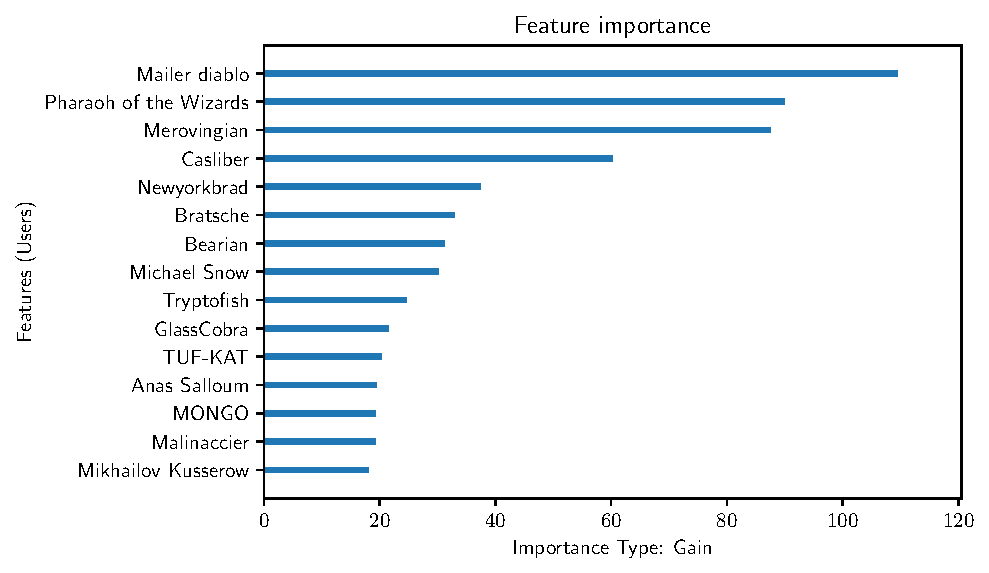
\includegraphics[width=\linewidth]{images/xgboost_features.pdf}
    \caption{XGBoost feature importance}
    \label{fig:xgboost-feat-importance}
\end{figure}

The second approach was formulating a set cover problem, every element of the ground set is a tuple of $(\text{voter},\text{election})$ and then we create a subset for each unique user. For every user we take each election they participated in and add the people who follow that user. This means that they voted after the user and also voted the same as the user. Therefore the set $S_u$ for every user is defined as 
\[
    S_{u} = \{(v,e) \mid \text{where } v \text{ voted the same after } u \text{ in election }e  \} 
\]
Then we order the subsets $S_u$ by their size and then try to find how much of the ground set we can cover by taking the top $k$ users' subsets. The ground set has $221,766$ elements, which is fewer than the total number of votes as there are certain elections where votes were duplicated or people voted twice. We see how the set cover increases as we increase the value of $k$ as seen in Figure~\ref{fig:set-cover}
\begin{figure}[!ht]
    \centering
    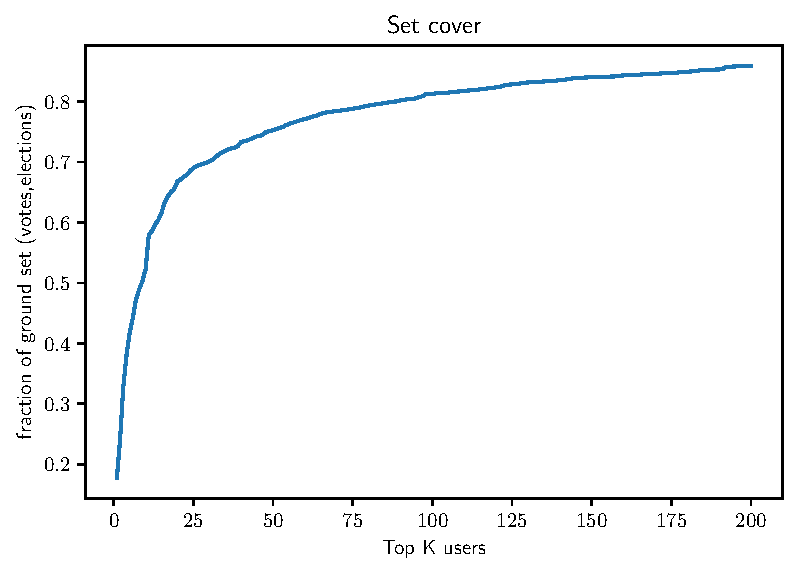
\includegraphics[width=\linewidth]{images/set_cover.pdf}
    \caption{Election set cover}
    \label{fig:set-cover}
\end{figure}
We see that with only $200$ top users we can cover nearly $85\%$ of the whole ground set. More interestingly we see that there is a knee around 25 users indicating that there is a small core of influential users. With the top $15$ users we have $60\%$ coverage. 

\begin{table}[!ht]
    \centering
    \caption{Top 10 influential users from XGBoost and the Set Cover models}
    \label{tab:top-10}
    \begin{tabular}{clr}
        \toprule
        Ranking&XGBoost&Set Cover\\
        \midrule
        1& Mailer diablo & Siva1979\\
        2&Pharaoh of the Wizards&Mailer diablo\\
        3&Merovingian&Newyorkbrad\\
        4&Casliber&Wizardman\\
        5&Newyorkbrad&Pedro\\
        6&Bratsche&Dlohcierekim\\
        7&Bearian&Juliancolton\\
        8&Michael Snow&Casliber\\
        9&Tryptofish&Acalamari\\
        10&GlassCobra&Fastily\\
        \bottomrule
    \end{tabular}
\end{table}
In Table~\ref{tab:top-10} we see many common users among the top 10 influential users from both approaches. This confirms the fact that in Wikipedia RfA elections there is a core set of voters who can be important in predicting the result of an election.

\section{Viscous Democracy and Model}
\label{sec:model}
Brief explanation of Viscous Democracy.
Use viscous democracy models using heuristic delegation functions on social network to predict elections separately

\section{Implementation}
\label{sec:implementation}
directed graph concepts and delegation function considerations.
Agony and hierarchy. local and global top k delegates.

\section{Results}
The quality of predictions using local or global important editors.
\label{sec:results}

\section{Conclusions}
How we can instead try and model individual voter behaviour. Find a more robust ML framework to learn an optimal delegation function.
\label{sec:conclusion}

\bibliography{ref}
\bibliographystyle{plain}

\section{Appendix}

\begin{figure*}[!ht]
    \centering
    \begin{subfigure}{0.49\textwidth}
        \centering
        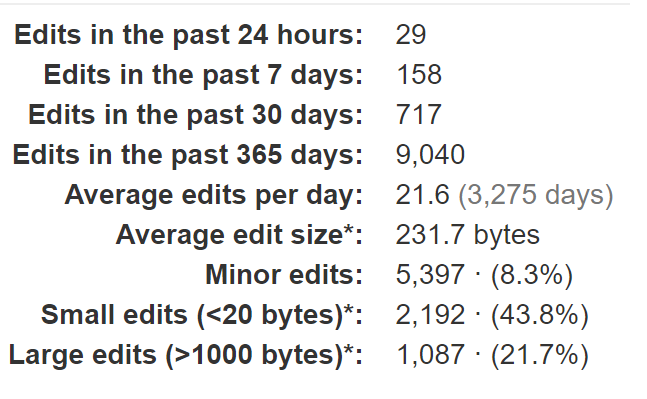
\includegraphics[width=\textwidth]{images/editor_stats.PNG}
        \caption{edit statistics}
        \label{fig:edit-stats}
    \end{subfigure}
    \begin{subfigure}{0.49\textwidth}
        \centering
        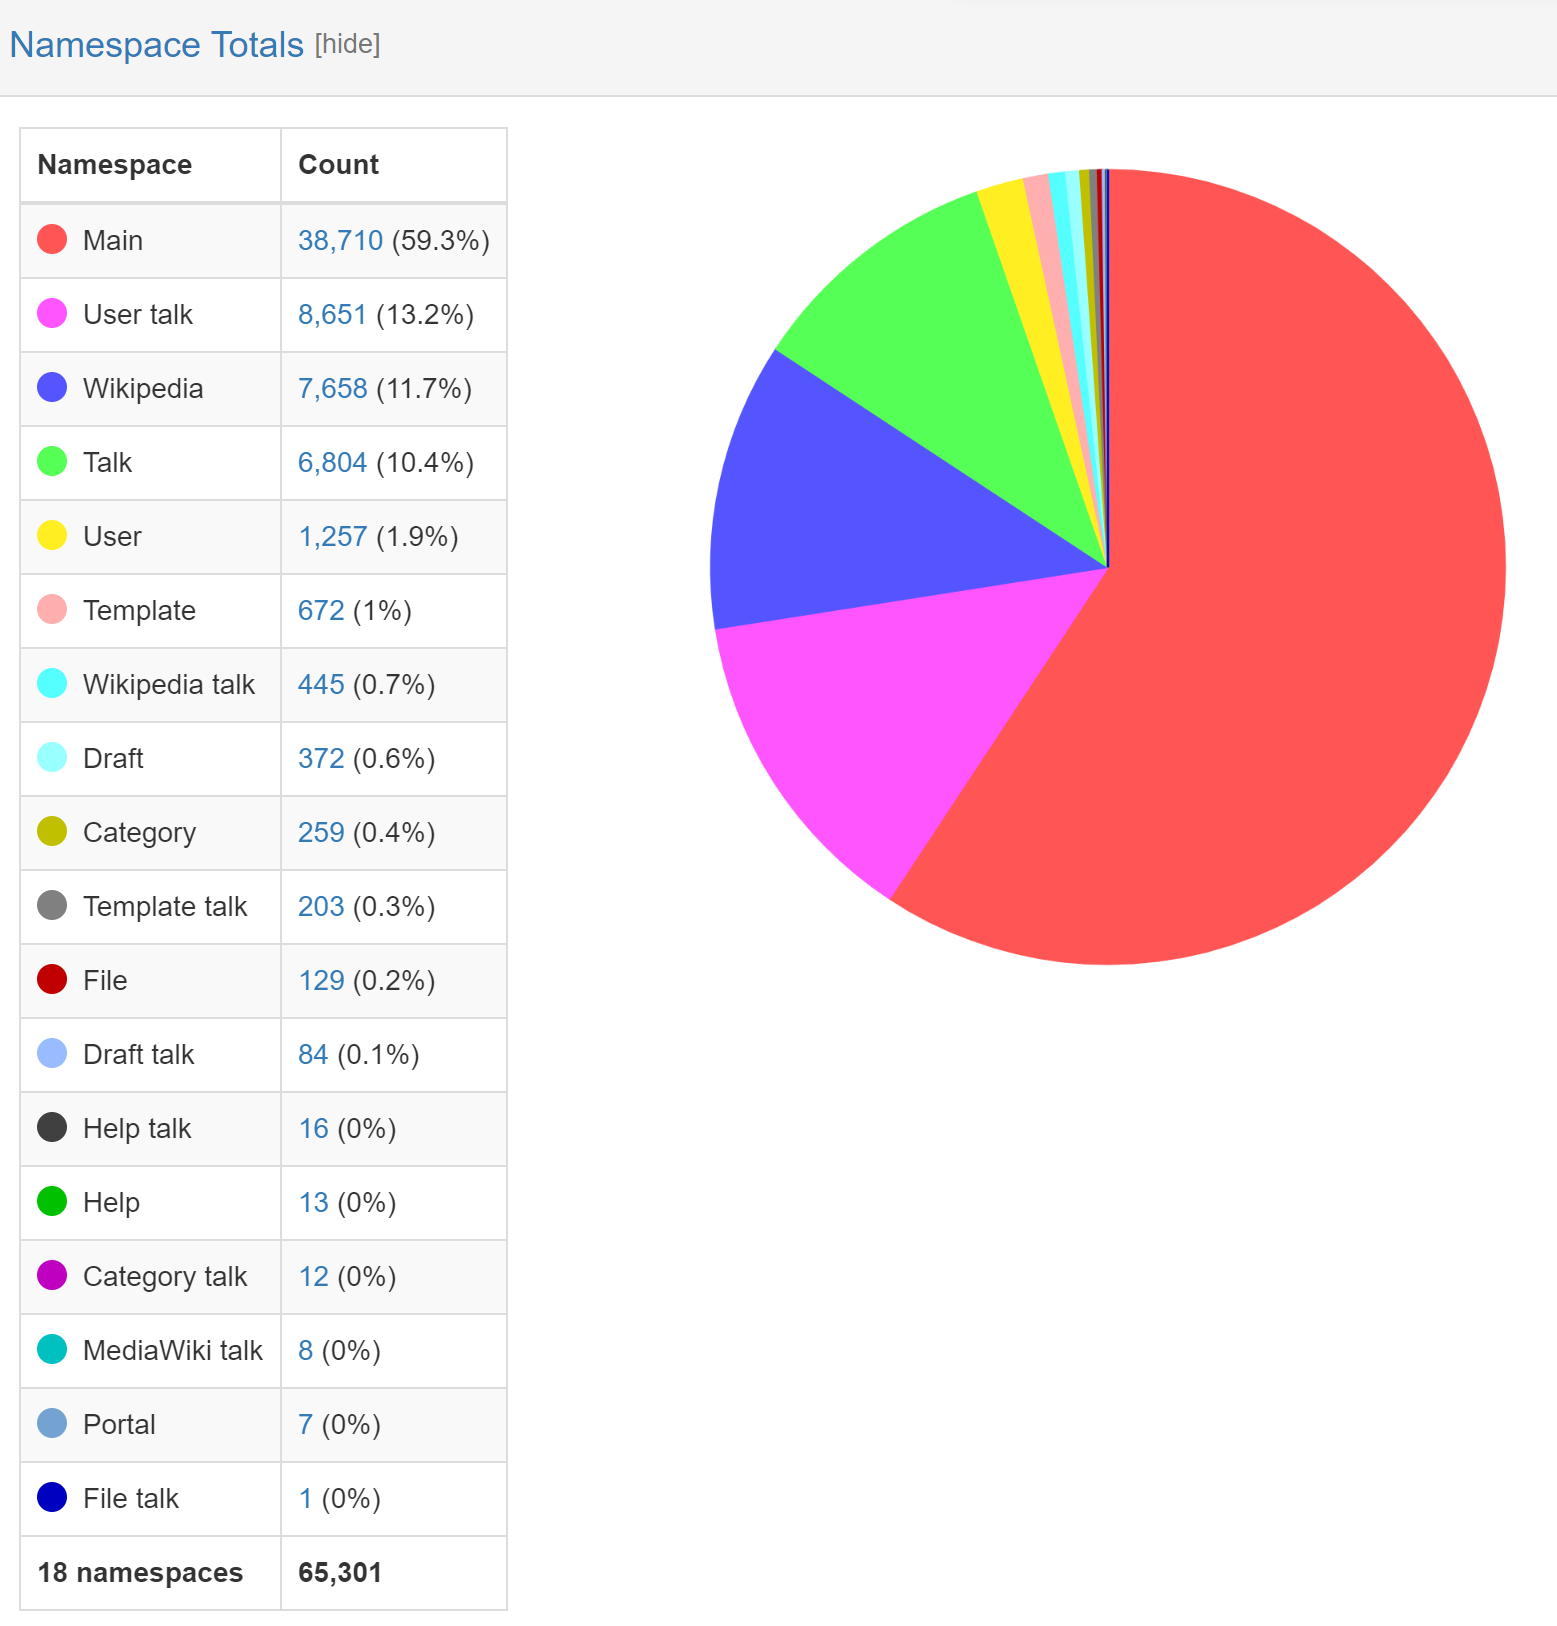
\includegraphics[width=\textwidth]{images/editor_totals.PNG}
        \caption{Edit namespace distribution}
        \label{fig:namespace-totals}
    \end{subfigure}

    \begin{subfigure}{0.49\textwidth}
        \centering
        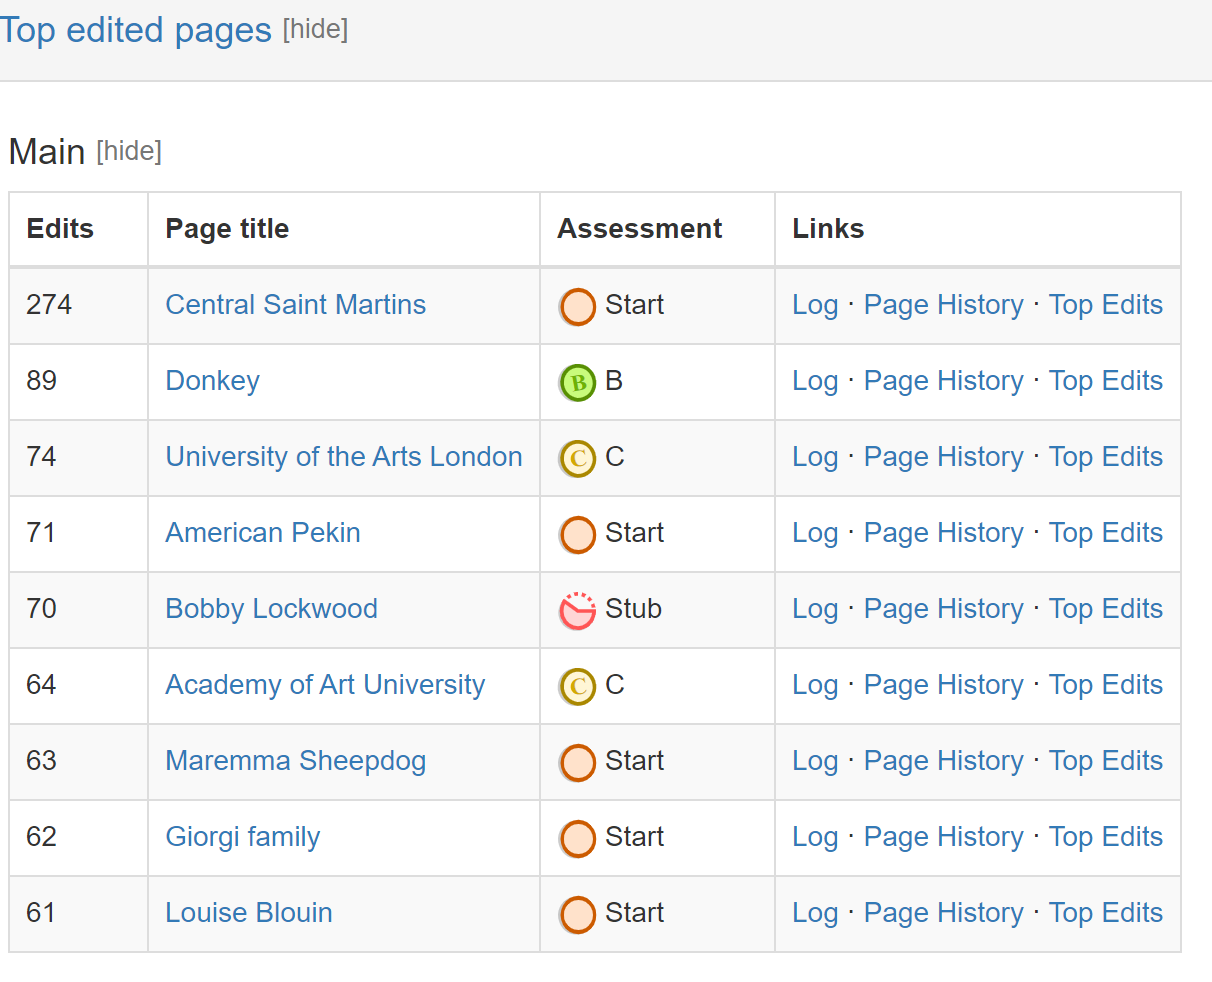
\includegraphics[width=\textwidth]{images/editor_top_edits.PNG}
        \caption{Top edited pages}
        \label{fig:top-edits}
    \end{subfigure}
    \begin{subfigure}{0.49\textwidth}
        \centering
        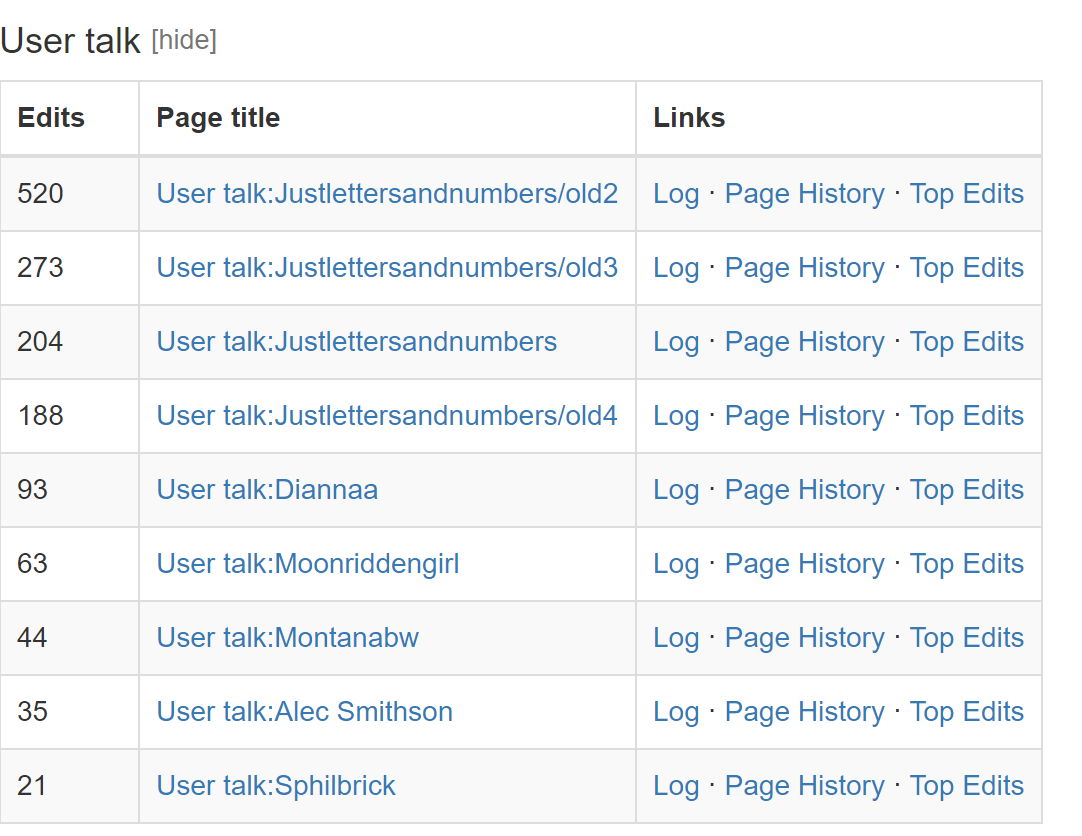
\includegraphics[width=\textwidth]{images/editor_user_talk.PNG}
        \caption{Top user talk pages edits}
        \label{fig:user-talk-edits}
    \end{subfigure}

    \caption{Edit summary of a Wikipedia user}
    \label{fig:edit-summary}
\end{figure*}

\begin{figure*}[!ht]
    \centering
    \begin{subfigure}{0.49\textwidth}
        \centering
        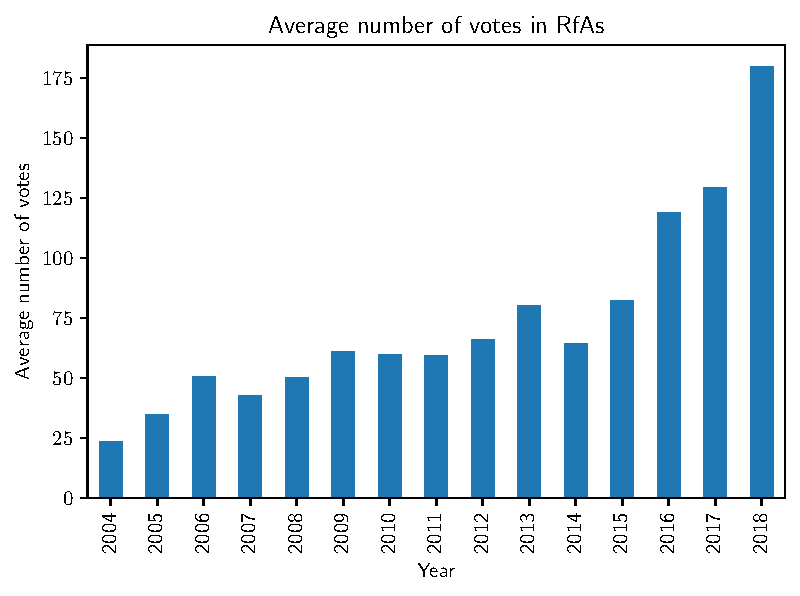
\includegraphics[width=\textwidth]{images/avg_votes.pdf}
        \caption{Vote distribution}
        \label{fig:vot-distribution}
    \end{subfigure}
    \begin{subfigure}{0.49\textwidth}
        \centering
        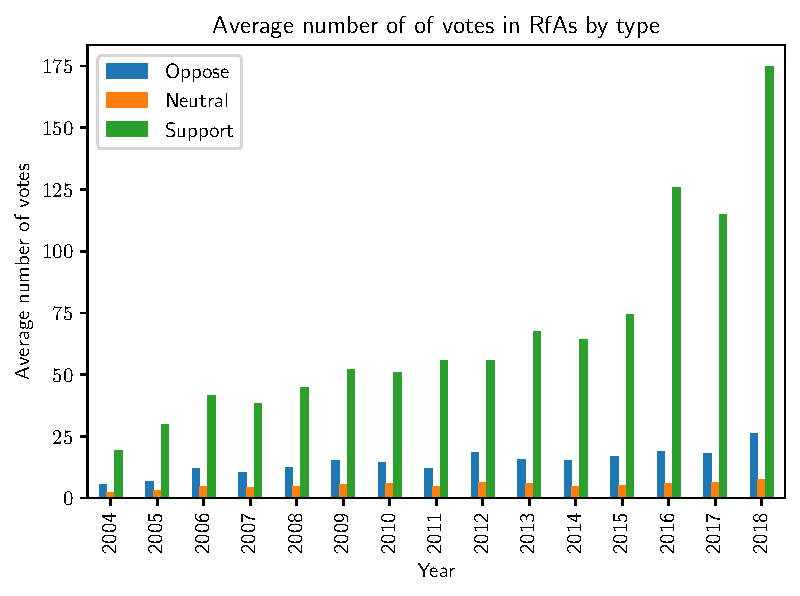
\includegraphics[width=\textwidth]{images/avg_votes_type.pdf}
        \caption{Vote distribution by tye }
        \label{fig:vote-type-distribution}
    \end{subfigure}
    
    \begin{subfigure}{0.49\textwidth}
        \centering
        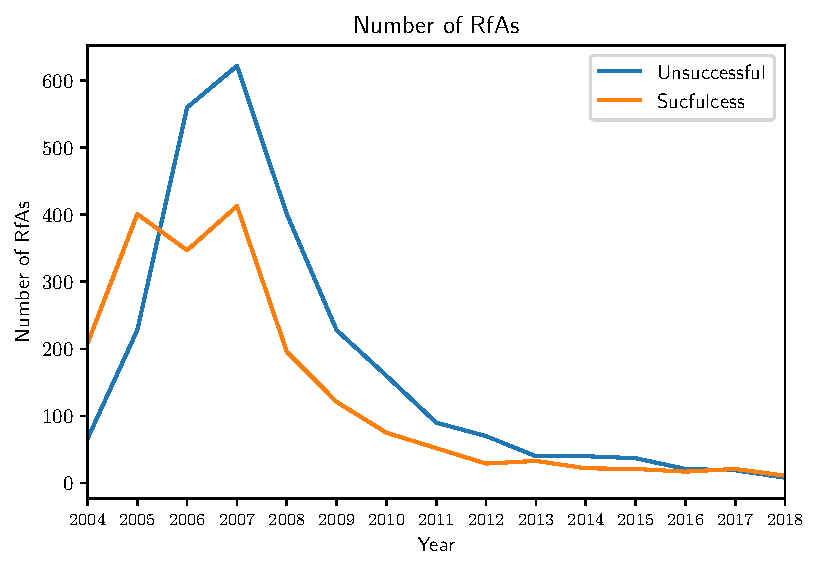
\includegraphics[width=\textwidth]{images/num_rfas.pdf}
        \caption{Number of RfA by year}
        \label{fig:num-rfas}
    \end{subfigure}
    \begin{subfigure}{0.49\textwidth}
        \centering
        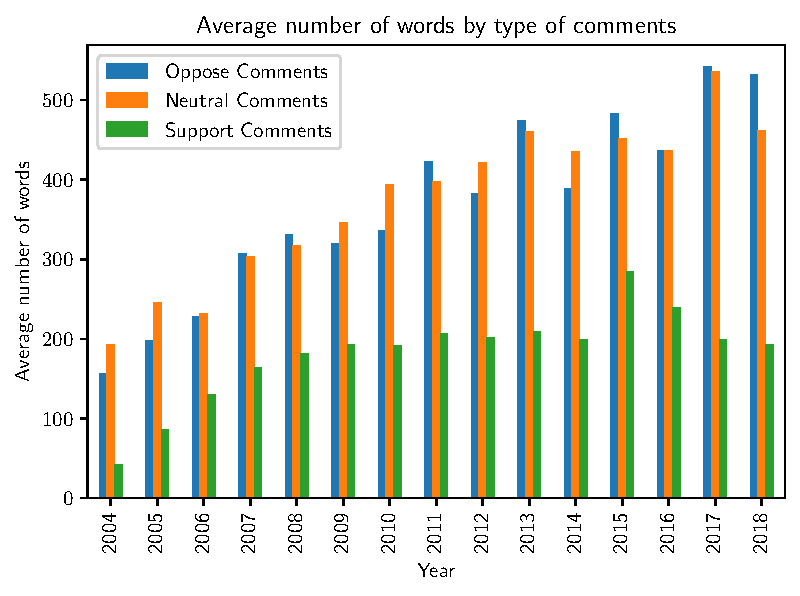
\includegraphics[width=\textwidth]{images/avg_comment_size_type.pdf}
        \caption{Comments distribution}
        \label{fig:comment-distribution}
    \end{subfigure}
\end{figure*}

\end{document}